%
\documentclass[12pt]{article}

% The usual packages
\usepackage{fullpage}
\usepackage{breakcites}
\usepackage{setspace}
\usepackage{endnotes}
\usepackage{float}
\usepackage{amsmath}
\usepackage{amsfonts}
\usepackage{amssymb}
\usepackage{rotating}
\usepackage{dcolumn}
\usepackage{longtable}
\usepackage{microtype}
\usepackage{graphicx}
\usepackage{hyperref}
%\usepackage[usenames,dvipsnames]{color}
\usepackage{url}
\usepackage{natbib}
\usepackage{framed}
\usepackage{epigraph}
\usepackage{lipsum}
\usepackage[font=small,labelfont=sc]{caption}
\restylefloat{table}
\bibpunct{(}{)}{;}{a}{}{,}

% Set paragraph spacing the way I like
\parskip=0pt
\parindent=20pt

% Define mathematical results
\newtheorem{lemma}{Lemma}
\newtheorem{proposition}{Proposition}
\newtheorem{theorem}{Theorem}
\newtheorem{claim}{Claim}
\newenvironment{proof}[1][Proof]{\begin{trivlist}
\item[\hskip \labelsep {\bfseries #1}]}{\end{trivlist}}
\newenvironment{definition}[1][Definition]{\begin{trivlist}
\item[\hskip \labelsep {\bfseries #1}]}{\end{trivlist}}
\newenvironment{example}[1][Example]{\begin{trivlist}
\item[\hskip \labelsep {\bfseries #1}]}{\end{trivlist}}
\newenvironment{remark}[1][Remark]{\begin{trivlist}
\item[\hskip \labelsep {\bfseries #1}]}{\end{trivlist}}
\DeclareMathOperator*{\argmin}{arg\,min}

% Set up fonts the way I like
\usepackage{tgpagella}
\usepackage[T1]{fontenc}
\usepackage[bitstream-charter]{mathdesign}

%% Set up lists the way I like
% Redefine the first level
\renewcommand{\theenumi}{\arabic{enumi}.}
\renewcommand{\labelenumi}{\theenumi}
% Redefine the second level
\renewcommand{\theenumii}{\alph{enumii}.}
\renewcommand{\labelenumii}{\theenumii}
% Redefine the third level
\renewcommand{\theenumiii}{\roman{enumiii}.}
\renewcommand{\labelenumiii}{\theenumiii}
% Redefine the fourth level
\renewcommand{\theenumiv}{\Alph{enumiv}.}
\renewcommand{\labelenumiv}{\theenumiv}
% Eliminate spacing around lists
\usepackage{enumitem}
\setlist{nolistsep}

% Create footnote command so that my name
% has an asterisk rather than a one.
\long\def\symbolfootnote[#1]#2{\begingroup%
\def\thefootnote{\fnsymbol{footnote}}\footnote[#1]{#2}\endgroup}

% Create the colors I want
\usepackage{color}
\definecolor{darkred}{RGB}{100,0,0}

\hypersetup{
pdftitle={The Heavy Tails of Electoral Data}, % title
pdfauthor={Dan Baissa and Carlisle Rainey}, % author
pdfkeywords={robust linear regression} {outliers} {leverage}
pdfnewwindow=true, % links in new window
colorlinks=true, % false: boxed links; true: colored links
linkcolor=darkred, % color of internal links
citecolor=darkred, % color of links to bibliography
filecolor=darkred, % color of file links
urlcolor=darkred % color of external links
}

% enable comments in pdf
\newcommand{\kelly}[1]{\textcolor{blue}{#1}}
\newcommand{\carlisle}[1]{\textcolor{magenta}{#1}}


\begin{document}

\begin{center}
{\LARGE \textbf{The Heavy Tails of Electoral Data}}\\\vspace{2mm}
{ \textbf{The Importance of Robust Estimators}\symbolfootnote[1]{We thank Bill Clark and Matt Golder for making their data available to us. The analyses presented here were conducted with \texttt{R} 3.1.0. All data and computer code necessary for replication are available at \href{https://github.com/carlislerainey/heavy-tails}{
github.com/carlislerainey/meaningful-inferences}
.}}\\\vspace{2mm}


\vspace{10mm}

Dan Baissa\symbolfootnote[2]{Dan Baissa is an M.A. student in the Department of Political Science, University at Buffalo, SUNY, 520 Park Hall, Buffalo, NY 14260 (\href{mailto:dkbaissa@buffalo.edu}{
kellymcc@buffalo.edu}
).}

\vspace{3mm}

Carlisle Rainey\symbolfootnote[3]{Carlisle Rainey is Assistant Professor of Political Science, University at Buffalo, SUNY, 520 Park Hall, Buffalo, NY 14260 (\href{mailto:rcrainey@buffalo.edu}{
rcrainey@buffalo.edu}
).}
\end{center}

\vspace{10mm}

% Abstract
{\centerline{\textbf{Abstract}}}
\begin{quote}\noindent
Researchers studying the consequences of comparative electoral institutions, as well as other areas of political and social science, often estimate linear regression models on continuous outcomes of interest using least squares. These outcomes include measures of the number of political parties, proportionality, and vote share, among others. While it is well known that least-squares estimates are often sensitive to single, influential data point, this knowledge has not led to appropriate practices when using least-squares estimators. We highlight the important using more robust estimators (at least as a robustness check) and discuss several approaches to detect, summarize, and communicate the influence of particular data points. We conclude with a reanalysis of Clark and Golder (2006) an show that their conclusions depend on several influential data points. Removing these data or using a robust estimator substantially weaken their key conclusions about the conditional relationship between social heterogeneity and electoral rules in influencing the number of political parties.
 \end{quote}

% Add quote to first page
% \epigraph{}

%\begin{center}
%Manuscript word count: 
%\end{center}

% Remove page number from first page
\thispagestyle{empty}

% Start main text
\newpage
\doublespace

\section*{Introduction}

Our goal in this manuscript, our goals are to (1) highlight powerful, robust alternatives to least-squares estimators, (2) provide concrete, practical advice to substantive researchers using linear models, and (3) provide a compelling example that shows the importance of robust estimators.

\section*{Is a BLUE Estimator the ``Best'' Estimator?}

The linear regression model can be written as $E(y | X) = X\beta + \epsilon$, where $y$ is an outcome variable of interest (usually roughly continuous), $X$ is a $n \times (k + 1)$ matrix containing a single column of ones and $k$ columns holding $k$ explanatory variables, $\beta$ is a $(k + 1) \times 1$ matrix of model coefficients, and $\epsilon$ is an $n \times 1$ matrix of errors. Researchers in political science commonly estimate this model with ordinary least squares (OLS) by minimizing the squared residuals, $\hat{\beta}^{OLS} = \argmin S(b)$, where $S(b) = \sum_{i = 1}^n(y_i - X_ib)^2$. That is, OLS estimators choose the estimate $\hat{\beta}$ that minimizes the sum of the squared residuals. Under the assumption that the errors $\epsilon_i$ follow independent and identical normal distributions with mean zero and unknown variance, the OLS estimator is the minimum variance unbiased estimator (MVUE).

Even if the errors do not follow independent and identical normal distributions, the Gauss-Markov Theorem guarantees the least-squares estimator is the best (i.e., minimum variance) \textit{linear} unbiased estimator if the errors have mean zero and constant (and finite) variance. However, this should provide little comfort to researchers because their is little statistical or substantive reason to restrict themselves to \textit{linear} estimators.

At first glance, one might take the linearity restriction under Gauss-Markov to refer to the structure of the model, such that $E(y | X) = X\beta$ falls into the class of ``linear'' regression models, but  $E(y | X) = e^{X\beta}$ does not. Indeed, this is the sense in which we use ``linear'' in the term ``linear regression.'' However, the ``linear'' restriction in the Gauss-Markov Theorem refers to a highly technical and obscure statistical criterion that requires that the estimates be a linear function of the outcome variables, so that $\hat{\beta}_j = \lambda_1 y_1 + \lambda_2 y_2 + ... \lambda_n y_n$, so that the weights $\lambda_i$ are allowed to depend on $X$, but not on $y$.\footnote{Formally, linearity requires that $\hat{\beta} = My$, where $M$ depends on the matrix $X$. For the case of least-squares, $M = (X'X)^{-1}X'$.} In other words, Gauss-Markov does not require a linear \textit{model} of the form $E(y | X) = X\beta$, but it does require a linear estimator of the form $\hat{\beta}_j = \lambda_1 y_1 + \lambda_2 y_2 + ... \lambda_n y_n$. 

However, we argue that restricting ourselves to linear estimators is unnecessary and unproductive. There is no statistical reason to restrict ourselves to linear estimators, except for mathematical convenience, and there are substantive reasons to reject this restriction. For example, if the researcher is aware that one case has a unusually large outcome variable (conditional on the explanatory variables), then the researcher might wish to weight that case less than the other, more typical cases so that one atypical case does not exert several times more impact on the estimates than other, typical cases. Indeed, substantive researchers might wish to attach zero weight to extremely unusual cases because these cases might be due to a different substantive process.

It is not often appreciated that if the errors do not follow independent and identical normal distributions, then the OLS is no longer the MVUE--other estimators might outperform OLS.

Many researchers simply assume a statistical model for which a MVUE is easily available for little or no substantive reason. Knowing that the assumed model (e.g., normality) is \textit{in}orrect, these researchers are using this model as an approximation. But if the model is an approximation, then the desirable statistical properties are not longer guaranteed (e.g., MVUE). With this in mind, it makes more sense to use a robust estimator with the following qualitative properties:
\begin{enumerate}
\item Approximately unbiased in typical sample sizes for the assumed model and small, plausible deviations.
\item Excellent efficiency under the assumed model, though perhaps not the best possible efficiency.
\item Excellent efficiency under small deviations from the assumed model
\item Reasonable efficiency and bias in typical sample sizes with large deviations from the assumed model. 
\end{enumerate}

Mathematically, this suggests that applied researchers should not necessarily restrict themselves to unbiased estimators or minimum variance estimators under an assumed model. Instead, a more desirable criterion might be the mean squared error of the estimate under a wide range of deviations from the assumed model. The ``best'' model for a social scientist might not be the optimal estimator for an assumed model, but an estimable that works reasonably well for the assumed model and many substantively plausible deviations. 

To see the importance of this in practice, we simulated 10,000 data sets 50 observations of variables $x$ and $y$, where the relationship between $x$ and $y$ is given by $y = x + \epsilon$, where $\epsilon$ follows a $t$ distribution with three degrees of freedom. Note that the $t_3$ distribution is symmetric, bell-shaped, and resembles the normal distribution, except it has slightly heavier tails. For each of these 10,000 data sets we used least-squares to estimate the slope of the relationship between $x$ and $y$. Because we simulated these data, we know that the Gauss-Markov assumptions hold. This means that least-squares is the \textit{best} linear unbiased estimator. The left panel of Figure \ref{fig:lts-illustration} shows the distribution of the estimated slopes using least squares.

But consider a least trimmed squares (LTS) estimator in which we minimize the smallest 90\% of the residuals. This method literally throws away data. Though it lacks the elegant theory of the least-squares estimate, the right panel of Figure \ref{fig:lts-illustration} shows that it is essentially unbiased and, compared to the least-squares more efficient (standard deviation about 18\% smaller), and has a much smaller mean squared error (about 32\% smaller) . By any reasonable standard, it is a better estimator than the least squares estimator. This improvement is dropped by expanding our focus to non-linear estimators. In this case, the LTS estimator is not linear because it places zero weight on the largest 10\% of the residuals and weights of one on the smallest 90\% of the residuals.

\begin{figure}[H]
\begin{center}
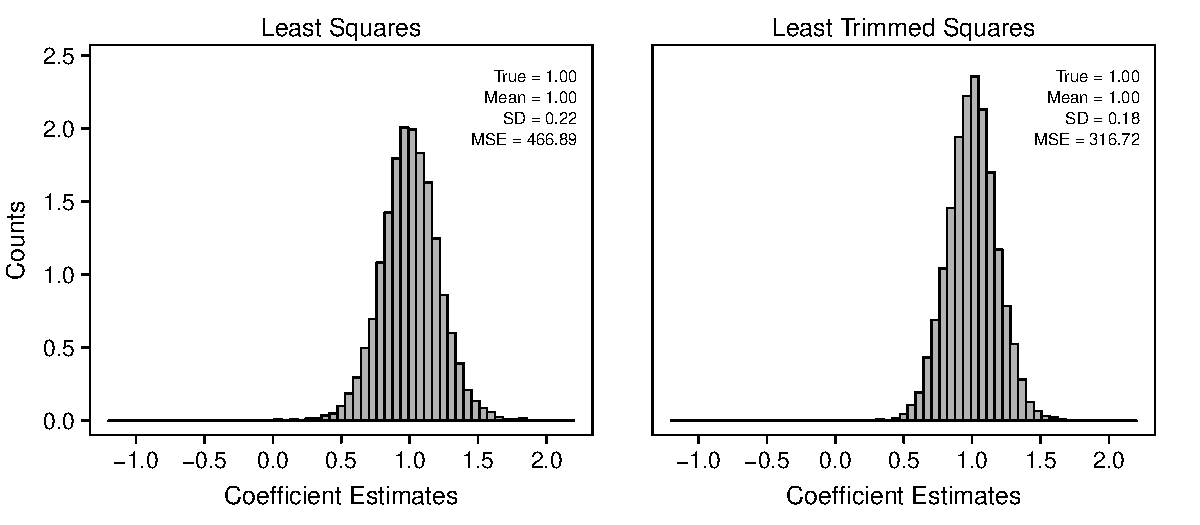
\includegraphics[scale = .7]{figs/lts-illustration.pdf}
\caption{caption here}\label{fig:lts-illustration}
\end{center}
\end{figure}

While the statistical properties of the least squares under the assumed normal-linear model are extremely well developed (e.g., MVUE), these properties are not nearly as well developed from robust alternatives. Some asymptotic results are available, but the closed-form theory is generally much weaker.

There has been a great deal of attention in the methodological literature to the sensitivity of standard errors to violations from the assumed model--and substantive scholars have paid attention. For example, White's (1980) seminal paper developing heteroskedasticity-consistent standard errors has received over 20,000 citations, making it one of the most cited papers in economics. Beck and Katz's (1995) introduction to panel corrected standard errors has received over 4,300 citations, making it one of the most cited political science papers ever.

On the other hand, there has been scant attention paid to the sensitivity of the estimates to similar violations. This is particularly problematic, since it makes little sense to find a good standard error for a poor estimate. Two papers in political science have addressed the issue of robust estimation. Western's (1995) introduces political scientists to robust estimators, but this work has been essentially ignored. The work is more broadly applicable than Beck and Katz (1995) and was published in the same year, but has received only 99 citations, or  about 2\% of the citations that Beck and Katz have received. Similarly, Demaris and Harden (2011) has received only one citation, and it comes from the authors themselves. Anderson's (2008) broad and accessible introduction to robust estimation methods has received only about 150 citations, most from outside political science.

This focus on obtaining reasonable standard errors at the expense of reasonable estimates can be seen in Gujarati (????, p. ??, ), a popular textbook for political science classes focusing on linear models. Though the text deals with robust standard errors in some detail, Gujarati writes (in a footnote):
\begin{quote}
In passing, note that the effects of departure from normality and related topics are often discussed under the topic of robust estimation in the literature, a topic \textit{beyond the scope of this book} [italics ours].
\end{quote}
Another popular textbook, Wooldridge (????) does briefly discuss robust estimators, though in a much more limited manner than his discussion of robust standard errors. Angrist and Pischke (2008), though, devote an entire chapter to robust standard errors and completely ignore robust estimation of model coefficients.

\section*{A Robust Alternative to Least Squares}

In spite of the scant attention paid to robust estimators in political science, statisticians have developed and refined many robust methods since the seminal work of Box (1953) and Huber (1964). Huber and Ronchetti (2009) provide a detailed review of these developments and Anderson (2008) provides an accessible introduction. 

Adjudicating among these many robust alternatives to least squares is beyond the scope of our paper, but, to fix ideas, we do introduce one robust estimator in detail which has several desirable properties--the MM-estimator. 

The MM-estimator, proposed by Yohai (1987). This estimator works extremely well if the assumed normal-linear model holds, though it is not quite as efficient as least squares. On the other hand, when the assumed normal-linear model does not hold, then the MM-estimator might be more efficient than the least squares estimator, perhaps substantially if the deviation is severe. MM-estimation actually combines three of robust estimation into an iterative procedure.

\begin{enumerate}
\item Calculate initial coefficient estimates and initial residuals using S-estimation.
\item Calculate the scale of the residuals using M-estimation.
\item Iterate the following until converge:
	\begin{enumerate}
	\item Update the coefficients using M-estimation with weights determined by the latest residuals.
	\item Calculate new residuals using the latest coefficients.
	\end{enumerate}
\end{enumerate}

We now discuss the details of S-estimation and M-estimation. Though the first step of the MM algorithm uses S-estimation, it is convenience to introduce the basic idea of M-estimation first.

\subsection*{M-Estimation}

While least squares yields the coefficients that minimize the sum of the squared residuals $\min \sum_{i = 1}^n \hat{e}_i^2$, M-estimation minimizes some other, less rapidly increasing function of the residuals $\min \sum_{i = 1}^n \rho(\hat{e}_i)$. Because the solution is not scale invariant, the residuals $\hat{e_i}$ are standardized by a robust estimate of scale $\hat{\sigma}_{(mad)}$, calculated using the median absolute deviation so that $\min \sum_{i = 1}^n \rho \left(\dfrac{\hat{e}_i}{\hat{\sigma}_{(mad)}}\right)$.



\singlespace
\bibliographystyle{apsr_fs}
%\bibliography{/Users/carlislerainey/Dropbox/papers/bibliography/bibliography.bib}
\bibliography{/Users/rcrainey/Dropbox/papers/bibliography/bibliography.bib}


\section*{Replication of Clark and Golder (2006)}

\begin{figure}[H]
\begin{center}
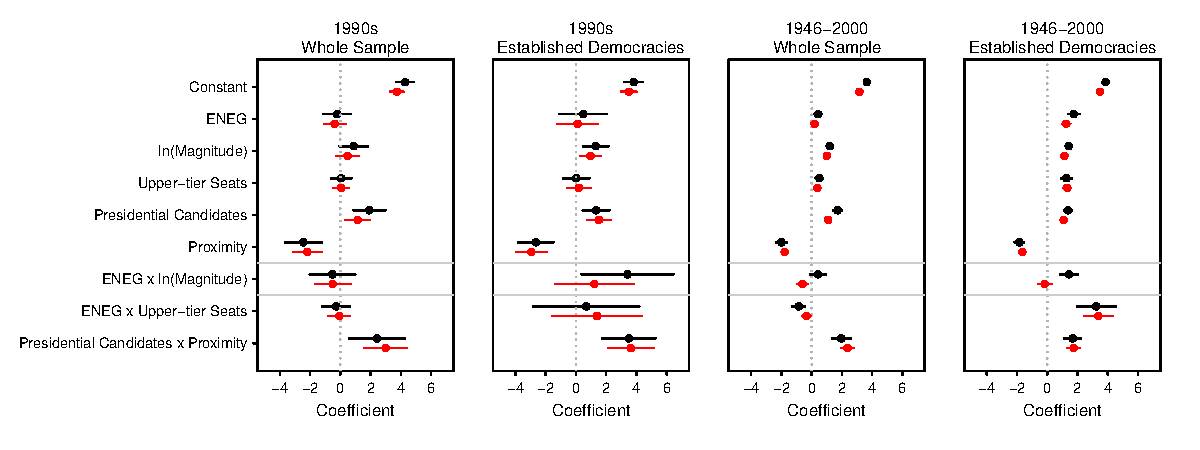
\includegraphics[scale = .8]{figs/cg-coef-plots.pdf}
\caption{Replication of Clark and Golder (2006) using MM-estimation with explanatory variables standardized to have mean zero and standard deviation one-half. The black lines and points show the OLS estimates and 90\% confidence intervals and the red lines and points show the MM estimates and confidence intervals. Notice that the coefficient for the product of the effective number of ethnic groups and the district magnitude changes drastically with the choice of estimator.}\label{fig:cg-coef-plots}
\end{center}
\end{figure}

\begin{figure}[H]
\begin{center}
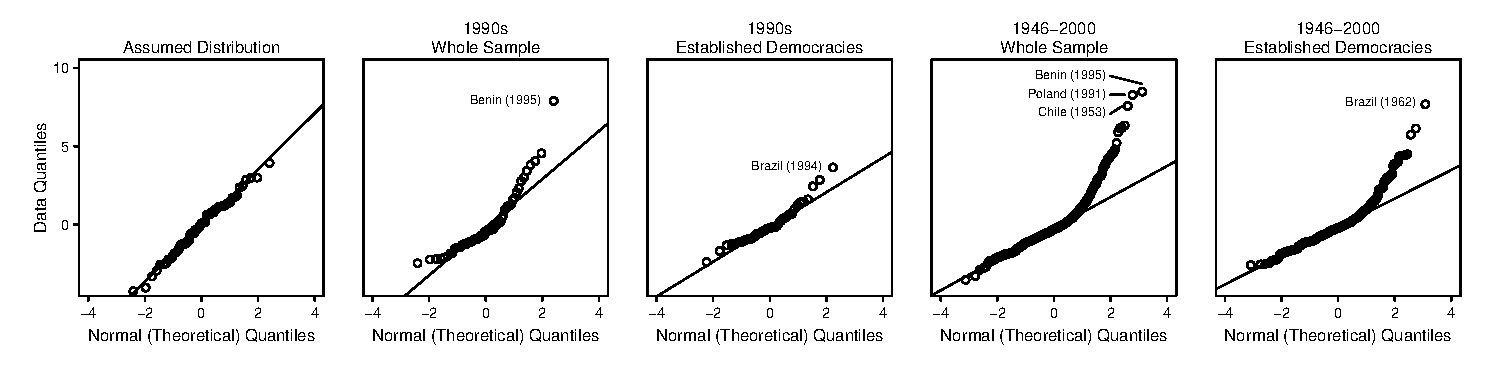
\includegraphics[width = \textwidth]{figs/cg-qq-plots.pdf}
\caption{caption here.}\label{fig:cg-coef-plots}
\end{center}
\end{figure}

\newpage
\doublespace
\begin{appendix}
\begin{center}
\textbf{{\LARGE Appendix}}\\\vspace{2mm}
\textbf{{\large The Heavy Tails of Electoral Data}}\\\vspace{2mm}

\end{center}
\section{}


\end{appendix}


\end{document}